
% -*- TeX:SI -*-
% slovene sub-mode for spell check
%%%%%%%%%%%%%%%%%%%%%%%%%%%%%%%%%%%%%%%%%%
% Glavni text
%%%%%%%%%%%%%%%%%%%%%%%%%%%%%%%%%%%%%%

\chapter[ABB RobotStudio]{Doma\v ca naloga \newline Programski paket za robotsko \newline simulacijo ABB RobotStudio}

\begin{mdframed}[backgroundcolor=green!20, shadow=true,roundcorner=8pt]
\vspace{-0.35cm}
\section{Cilji vaje}
\begin{itemize}
\item spoznavanje dela z off-line okoljem za programiranje robotov ABB
\item umestitev robota in CAD delovnih objektov  v navidezno okolje
\item uporaba novega vrha robota v obliki novega CAD orodja
\item definiranje uporabniških koordinatnih sistemov, ki pripadajo obdelovancu
\item uporaba ukazov za linearno in krožno premikanje robota po obliki obdelovanca
\item priprava programa za vodenje robota v navideznem okolju s pomočjo točk definiranih z modelom obdelovanca
\item simulacija izvajanja programa v navideznem okolju
\item prenos programa iz navideznega okolja na realni robot ABB

\end{itemize}
\end{mdframed}

\section{Uvod}
\emph{ABB RobotStudio} je simulacijski programski paket, ki omogoča grafično
prostorsko simulacijo delovanja robotskih celic. Programski paket omogoča:

\begin{itemize}
\item\vspace*{-0.35cm} prostorsko modeliranje robotske celice, ki
lahko vključuje več robotov hkrati, periferijo ter ostale naprave v
celici. Model robota vključuje kinematični model robota, ki omogoča
vodenje v zunanjih in v notranjih koordinatah, kakor tudi model
programskega jezika in okolja krmilnika. \item\vspace*{-0.35cm}
načrtovanje trajektorij gibanja (pri načrtovanju poti je v primerjavi
z realnim sistemom dobrodošla možnost načrtovanja glede na geometrijo
predmetov v celici), \item\vspace*{-0.35cm} simulacijo delovanja,
\item\vspace*{-0.35cm} kreiranje robotskega programa.
\end{itemize} Namen in prednosti uporabe robotske simulacije
so:
\begin{itemize}
\item\vspace*{-0.35cm} Vizualizacija ideje o avtomatizaciji določene
delovne naloge. \item\vspace*{-0.35cm} Preverjanje ustreznosti
različnih tipov robotov še pred odločitvijo o nakupu, kar omogoča
knjižnica modelov robotov. \item\vspace*{-0.35cm} Off-line
programiranje: Robotski program se v tem primeru razvije na
simulacijskem paketu na modelu celice, za prenos na realno celico v
proizvodnji pa je potreben le minimalen čas zaustavitve.
\end{itemize}

\vspace{15mm}

{\bf Zagon programskega paketa RobotStudio:}

\noindent Robot studio zaženite s klikom na ikonco v namizju ali
pod
\newline \textit{Start>Programs>ABB Industrial IT>Robotics IT>Robot
Studio}

\newpage
\section{Delovno okolje RobotStudio}

Izbira pogleda v delovnem okolju:
\begin{itemize}
\item\vspace*{-0.35cm} kolešček miške: približevanje/oddaljevanje
(zoom in/zoom out)

\item \vspace*{-0.35cm} srednja tipka miške (STM) + desna tipka miške
(DTM): rotacija točke pogleda

\item \vspace*{-0.35cm} tipka Control + leva tipka miške (LTM):
translacijski pomik točke pogleda.
\end{itemize}

\noindent Izbira objektov: krivulja, površina, objekt, skupina
objektov, ...

\noindent Lovljenje kurzorja na: mreži, v centru, v sredini med
oglišči, na oglišču, na robu \newline (enako z \textit{View>Snap
Mode})
\newline Ob hkratnem držanju tipke \textit{Alt} se prikazuje
trenutna izbira.


\begin{figure}[h]
\centering
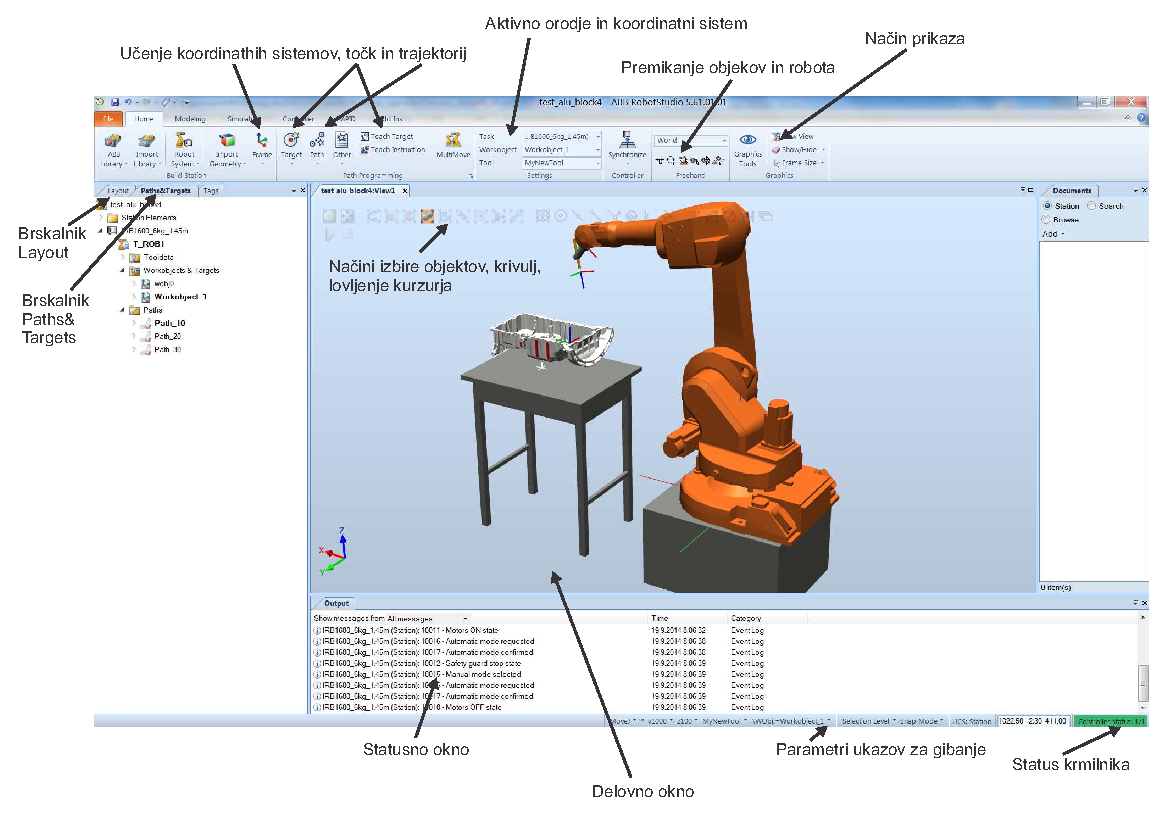
\includegraphics[width=1.0\columnwidth]{Delovno_okoljeRS_v6.eps}
  \caption{\label{figure1} Delovno okolje simulacijskega paketa RobotStudio}
\end{figure}


\newpage
\section{Načrtanje simulacijskega modela robotske celice}

Ustvari lokalno mapo \emph{D:$\setminus$Vaje$\setminus$or$\setminus$RobotStudio$\setminus$ImePriimek} (pri tem predlagamo, da namesto \v sumnikov uporabite \v crke brez stre\v sic). V lokalno mapo skopirajte zip datoteko \emph{PERIFERIJA.zip} iz mape \newline \emph{S:$\setminus$or$\setminus$RobotStudio$\setminus$PERIFERIJA} in jo odpakirajte. V datoteli se nahajajo robotska postaja, ki vsebuje robota, ki je enak realnemu robotu v laboratoriju LRBT (\emph{IRB1600 6kg 1.45m}) na podstavku in 3d modeli komponent, ki jih boste vklju\v cili v robotsko celico. To bo va\v sa lokalna kopija datotek, ki jih potrebujete za doma\v co nalogo. Odprite RobotStudio, v \emph{File} zavihku izberite  \emph{Open}, ter odprete  \emph{IRB1600.rspag} datoteko. Odpre se okno \emph{Unpack} \& \emph{Work}, kliknite \emph{Next}. Nato v \emph{Target folder} izberete va\v so mapo \emph{D:$\setminus$Vaje$\setminus$or$\setminus$RobotStudio$\setminus$ImePriimek} in izberete \emph{Next}. V naslednjem oknu ponovno izberete \emph{Next} in nazadnje \emph{Finish}. Sedaj po\v cakate, da se RobotStudio Package odpakira, ko lahko izberet \emph{Close}. Sedaj se odpre delovni prostor z robotom IRB\_1600\_6kg\_1.45m. Nadaljujete z ustvarjanjem orodja.

Sedaj lahko shranite postajo \emph{File>Save Station}. Postajo vam bo shranilo pod format datoteke \emph{rsstn}. To datoteko boste lahko urejali le na istem ra\v cunalniku, saj se v to datoteko na shranijo vse knji\v znjice, ki jih sicer potrebujete za odpiranje postaje na drugem ra\v cunalniku. \v Ce \v zelite postajo prenesti na drug ra\v cunalnik, je potrebno postaja prej NUJNO zapakirati. V \emph{File} zavihku izberete \emph{Share}, nato pa \emph{Pack and Go}. Postajo vam bo shranilo v \emph{rspag} datoteko, ki jo lahko preneste na drug ra\v cunalnik. Ko boste doma kon\v cali doma\v co nalogo jo morate nujno shraniti s \emph{Pack and Go}, sicer je ne bomo morali v laboratoriju, ko nam boste doma\v co nalogo \v zeleli predstaviti, odpakirati in pregledati.

\noindent \textbf{Kreirajte orodje} robota.
\begin{enumerate}
	\item Najprej naložite geometrijski model
	orodja preko \emph{Modelling>Import Geometry>Browse for Geometry...} - izberite \emph{orodje3.sat}.
	\begin{description} \item (Objekt se po
		vključitvi nahaja pod robotom in zato ni viden. \textbf{POZOR! Predno ga premikate oz.
			izvlečete izpod robota, ga obvezno definirajte kot orodje.} Torej nadaljujte z naslednjim korakom.)
	\end{description}
	\item Nato geometrijski model definirate kot orodje: \emph{Modelling>Mechanism>CreateTool} (zavihek \emph{Modelling}, orodno polje \emph{Mechanism}, ikona \emph{CreateTool}).
	\begin{itemize}
		\item izberite opcijo \emph{Use Existing} in izberite
		\emph{orodje3},
		\item vnesite položaj težišča: (-1.27, -1.27, 39.35) mm, maso 1 kg, vztrajnostni moment lahko izberete poljubno (recimo 0.1, 0.1, 0.1), \textbf{POZOR! RobotStudio razlo\v cuje med znakom za piko . in znakom za vejico , pri zapisu decimalnih \v stevil } zato je potrebno na nekaterih ra\v cunalnikih uporabiti za decimalni zapis pike, na drugih pa vejice. \v Ce vam torej ne uspe ustvariti orodja, je morda vzrok, da ste uporabili napa\v cni znak za zapis decimalnih \v stevil. Na novo odpakirajte \emph{PERIFERIJA.zip} in odprite popolnoma sve\v zo kopijo postaje.
		\item v naslednjem oknu določite vrh orodja tj. \emph{Tool Center Point} ali TCP, ki je določen glede na koordinatni sistem orodja. Vnesete koordinate (55.53, 0, 116.21) in rotacijo $50^o$ okoli osi \emph{y}. 
		\item Definirano točko dodate v spisek točk s pušcico v desno in zaključite.
		%    \item \vspace*{-0.cm} \hspace{0.5cm}- definicijo orodja je možno popravljati v brskalniku \newline \emph{Layout>Celica>MyNewTool DTM>ModifyToolData},
		\item definirano orodje pripnite na robot: v zavihku \emph{Layout} z miško primite
		\emph{MyNewTool} in ga povlecite na objekt $IRB1600\_6\_\_145\_01$. Odgovorite pozitivno na vprašanje ali želite posodobiti trenutno pozicijo, s čimer je orodje pripeto na zadnjem robotskem segmentu.
		%  \item \vspace*{-0.cm} \hspace{0.5cm}- orodje še pravilno orientirajte in sicer tako, da ga pod Elements izberete in z \emph{DTM>Rotate} orodje zavrtite za $180^o$ okoli $z$ osi lokalnega koordinatnega sistema.
	\end{itemize}
\end{enumerate}

Načrtan model robotske celice shranite.

%če sistema niste shranili, potem nadaljujte z navodili na strani \pageref{Prazna stran}. Sicer pa vedno lahko shranite sistem in nadaljujete z %navodili od tukaj naprej.

\noindent V prostor robotske celice \textbf{dodajte mizo} na katero bo postavljen obdelovanec preko \emph{Modelling>Import Geometry>Browse for Geometry...} - v mapi \newline
\emph{D:$\setminus$vaje$\setminus$or$\setminus$RobotStudio$\setminus$PERIFERIJA}
%\emph{(oz.//robo/student/or/RobotStudio/PERIFERIJA)}
izberite \emph{miza.sat}.
\begin{itemize}
\item  miza se znajde na ravnini
nič robotskega krmilnika, zato jo premaknite na 0 mm: v
zavihku \emph{Layout} na levi strani izberite mizo in z desno
tipko na miški (DTM) izberite \emph{Poisiton>Set Position}, z = -370 mm,
\item mizo premaknete po x na \emph{800 mm},
\item mizo zavrtite po z osi \textbf{lokalnega koordinatnega sistema} (\emph{Reference>Local}) za \emph{90 stopinj}.
\end{itemize}

Na mizo namestite obdelovanca:
\begin{itemize}
\item  v primeru uvoda odprite \textbf{kocko} (\emph{kocka.sat}). Kocka bo na višini \emph{483.5 mm} in premaknjena po x na \emph{960 mm} poravnana z ravnino mize.
\item ko boste delali doma?o nalogo pa na mizo namestite \textbf{aluminijasti blok} (\emph{alu\_blok.sat}). Postavite ga na pozicijo \emph{x=910, y=-40, z=570 mm}, ter zavrtite v oseh \textbf{lokalnega koordinatnega sistema} (\emph{Reference>Local}) \emph{x=90, y=0, z=180 stopinj}.
\end{itemize}


%\newline

\noindent Objekte v celici lahko premikate na več načinov: v
zavihku \emph{Layout} izberite objekt, ki se nahaja pod \emph{Components} in nato:
\begin{itemize}
   \item  objekt premikate s pomočjo ikonc \emph{Move} in \emph{Rotate} (ki se nahajajo v zavihku \emph{Home} v orodnem polju \emph{Freehand}) ter puščic, ali
    \item  objekt premikate tako, da v brskalniku izberete \emph{DTM>Set Position, >Rotate} ali >\emph{Place}
\end{itemize}




\section{Ročno vodenje robota}

Robot lahko ročno vodite na več načinov:

\begin{enumerate}
\item \vspace*{-0.2cm} Preko orodnega menija \emph{Freehand} z
\emph{Jog Joint}, \emph{Jog Linear} ali \emph{JogReorient} in robot
premikate z uporabo puščic.

%\item \vspace*{-0.2cm} Isto funkcionalnost kot pri 1 dosežete
%preko \emph{Jog Reorient} ali \emph{Jog Linear} ikonc.

\item \vspace*{-0.2cm}  V zavihku \emph{Layout} izberete robot
\emph{IRB1600\_5\_145\_\_01} in z \emph{DTM} izberete
\emph{Mechanism Joint Jog} ali \emph{Mechanism Linear Jog}. V teh
dveh načinih lahko ročno vnašate želene koordinate ali premikate
robot po korakih.

\end{enumerate}


\textbf{Naloga:} preizkusite vse možne načine ročnega vodenja!

\section{Kreiranje uporabniškega koordinatnega sistema (ang. Work object)}

Uporabniški koordinatni sistem oz. delovni objekt, ki je v bistvu koordinatni
sistem pripet na določen objekt, kreiramo z namenom, da točke gibanja učimo
relativno glede na ta objekt.  V primeru, da se objekt premakne, ostanejo
naučene trajektorije gibanja relativno glede na objekt enake.
\newline

\noindent Delovni objekt kreiramo tako, da najprej kreiramo koordinatni sistem
in sicer s pomočjo orodne ikonce \emph{Frame>Frame from Three Points} (nahaja se v orodnem polju \emph{Create}) s čimer
se odpre okno \emph{Create Frame}:
\begin{description}
\item \vspace*{-0.2cm} - izberemo opcijo Three Point, ki omogoča
definicijo koordinatnega sistem s tremi točkami. Prva točka
predstavlja izhodišče, druga določa smer $x$ osi, tretja pa smer $y$
osi. Kadar definiramo lego koordinatnega sistema glede na nek objekt
je najprimerneje, da koordinate točk določimo v t.i. \emph{Snap}
načinu:
\begin{itemize}
    \item \vspace*{-0.2cm} kurzor postavimo v okno za vpis koordinat točke,
    \item \vspace*{-0.2cm} v delovnem oknu izberemo
    način lovljenja koordinat v ogljiščih objekta \emph{Snap End},
\item \vspace*{-0.2cm} z držanjem tipke \emph{Alt} dobimo prikaz
lovljenja kurzorja glede na objekt,
    \item \vspace*{-0.2cm} z miško izberemo želeno ogljišče in koordinate se zapišejo v okno za definicijo koordinatnega sistema.
\end{itemize}

\item \vspace*{-0.2cm} - ko določimo koordinate vseh treh točk,
zaključimo definicijo koordinatnega sistema s \emph{Create} in dobimo
izrisan nov koordinatni sistem.

\item \vspace*{-0.2cm} - koordinatni sistem pretvorimo v delovni
objekt \emph{Workobject} z izbiro imena koordinatnega sistema v
zavihku \emph{Layout} ter z izbiro \emph{DTM>Convert Frame to
Workobject}

\item \vspace*{-0.2cm} - ustvarjen delovni objekt se znajde v
zavihku \emph{Paths\&Targets}

\item delovni objekt bomo sedaj povezali z objektom kocka. S tem se bo ob premikanju objekta kocka, s kocko ustrezno premikal tudi delovni objekt. V zavihku \emph{Paths\&Targets} z izbiro \emph{DTM>Attach to} odprete okno v katerem izberete objekt \emph{kocka} in negativno odgovorite na vprašanje, če želite posodibiti trenutno pozicijo.
\end{description}

\begin{figure}[h]
\centering\label{fig:kocka}
\includegraphics[width=0.7\columnwidth]{RStudio_workobject.eps}
  \caption{ Uporabniška koordinatna sistema na robu mize in robu kocke}
\end{figure}


\noindent Delovni objekt lahko tudi direktno kreiramo pod zavihkom \emph{Home} s klikom na ikono \emph{Other}
in \emph{Create Workobject}:
\begin{description}
\item \vspace*{-0.2cm} - delovni objekt poljubno poimenujemo ali
pustimo nespremenjeno,

\item \vspace*{-0.2cm} - opcijo \emph{Robot holds workobject}
izberemo \emph{False},

\item \vspace*{-0.2cm}- opcijo \emph{Moved by mechanical unit}
pustimo prazno,

\item \vspace*{-0.2cm}- opcijo \emph{Programmed} izberemo \emph{True}
(ker ne gre za premikajoči se koordinatni sistem), \item
\vspace*{-0.2cm} - določimo koordinatni system pod \emph{User Frame}:
\begin{itemize}
    \item \vspace*{-0.2cm} pozicijo in orinetacijo določimo tako, da izberemo izpis koordinat, kliknemo v eno, in nato v celici kliknemo na želeno točko (prej pravilno izberemo \emph{Snap
    mode}),
    \item \vspace*{-0.2cm} orientacijo koordinatnega sistema določimo ali z vnosom želenih zasukov ali pa z opcijo \emph{Frame by points}, kjer z izbiro treh točk določimo zasuk koordinatnega
    sistema,
    \item \vspace*{-0.2cm} izberemo \emph{Create} in dobimo izrisano nov koordinatnih
    sistem.
\end{itemize}
\end{description}


\noindent Delovni objekt lahko popravljamo tako, da ga v zavihku
\emph{Paths\&Targets} izberete in preko \emph{DTM>Modify Workobject}
popravite želene parametre.

\vspace{1cm}

\noindent \textbf{Naloga:} Pri uvodu v vajo določite delovni objekt na objektu z izhodiščem v enem od vogalov kot prikazuje slika \ref{fig:kocka}.

\begin{figure}[h]
\centering\label{fig:kalibSpice}
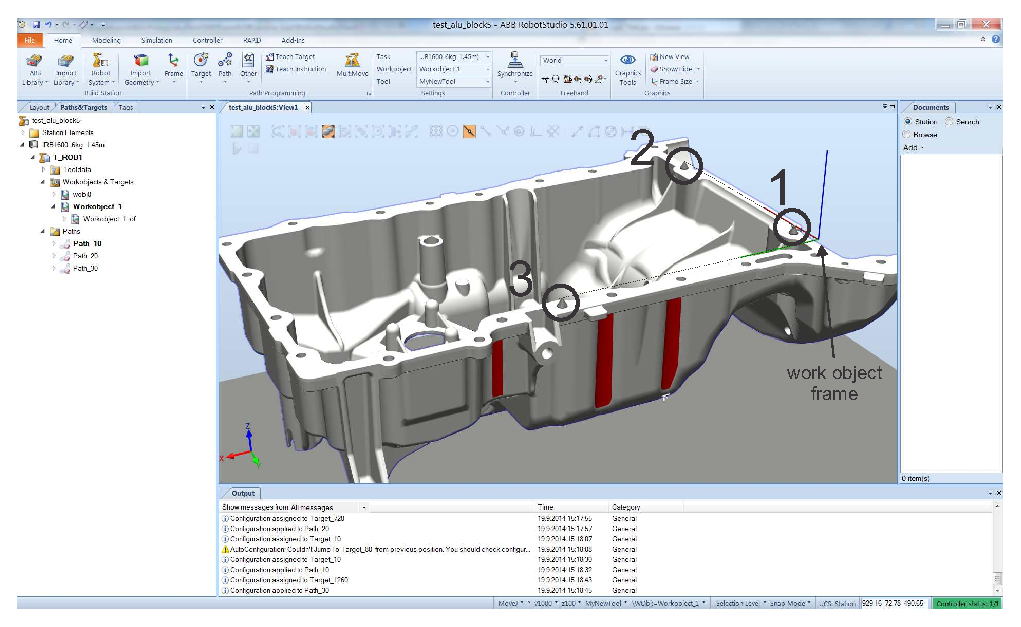
\includegraphics[width=0.9\columnwidth]{alu_blok_frame.eps}
  \caption{Uporabniška koordinatna sistema na modelu aluminijastega bloka.}
\end{figure}

Pri vaji pa postavite posamezne točke na kalibracijske špice, ki se nahajajo na modelu aluminijastega bloka kot prikazuje slika \ref{fig:kalibSpice}.

\comment{

\section{KREIRANJE UPORABIŠKEGA KOORDINATNEGA SISTEMA (User
Coordinate System - UCS)}

Uporabniški koordinatni sistem definiramo, kot poljubni koordinatni
sitem v prostoru. Uporaben je, če želimo določevati položaj točk ali
lego nekega objekta gleda nanj. Npr. če v zavihku \emph{Layout}
izberemo določen objekt in z \emph{DTM>Set as UCS} določimo
koordinatni sistem kot je koordinatni sistem tega objekta. Glede nanj
lahko določamo lego točk.

}

\section{Kreiranje ciljnih točk}

Ciljne točke (ang. Target points - TP) so lege vzdolž katerih se robot
giblje. Ciljne točke je možno kreirati na več načinov:

\begin{enumerate}
\item  Robot \textbf{ročno vodimo} v želen položaj z uporabo enega od
opisanih načinov in v želenem položaju izberemo ikono \emph{Teach
Target} (zavihek \emph{Home}, orodni meni \emph{Path Programming}). Na ta na?in u?imo to?ke, ki se ne nahajajo na obdelovancu. Vedno je potrebno robota pripeljati nad obdelovanca, zato da se robot brez trkov varno pribli?a obdelovancu. V tem primeru uporabimo tak na?in u?enja to?k. Robota ro?no prestavimo v neko to?ko nad obdelovancem od koder bo gibanje robota do obdelovanca varno. 

V zavihku \emph{Paths\&Targets} se pojavi nova točka v delovnem
objektu \emph{(Paths\&Targets>Workobject)}, ki je trenutno izbran kot
aktiven, kar pomeni, da so koordinate točke določene glede na ta
delovni objekt (ta trenutek lahko izbiramo med \emph{wobj0}, ki je
bazni ks in \emph{Workobject\_1}, ki je ks mize oz. objekta).

\item Lahko pa točke učimo \textbf{glede na geometrijo} objektov, ki
so prisotni v celici, in sicer:

\begin{itemize}
\item izberemo želen način lovljenja kurzorja (\emph{Snap mode}).
Namig: s hkratnim držanjem tipke \emph{Alt} vidimo ulovljen položaj
kurzorja.

\item točko - TCP kreiramo s \emph{Target>Create Target}, odpre se
nastavitveno okno:

\begin{description}
       \item - izberemo koordinatni sistem, glede na katerega definiramo točko
       \emph{Reference},
       \item - izberemo pozicijo, tako da kliknemo v koordinato in nato kliknemo na
       objekt,
       \item - orientacijo lahko ročno vpišemo ali jo popravljamo
       kasneje,
       \item - novo točko, ki se pojavi v delovnem objektu, kreiramo s
       \emph{Create},
\end{description}

       \item  nova točka, ki je določena preko geometrije nima določene konfiguracije robota, kar je potrebno naknadno določiti. (To se vidi v zavihku \emph{Paths\&Targets}, kjer se pri točki
       nahaja rumen trikotnik s klicajem)

    \item orientacijo orodja v naučeni točki preverimo tako, da v zavihku \emph{Paths\&Targets} izberemo točko in z \emph{DTM>View Tool at Target} dobimo prikaz lege orodja v točki. Vključimo tudi opcijo \emph{View Robot at Target} in s tem dobimo prikaz lege robota v točki.

    \item  orientacijo v naučeni točki  popravljamo z \emph{Paths\&Targets>DTM>Modify Target}, \emph{Rotate} ali ostale opcije, npr. \emph{Set Normal to Surface}, ali \emph{Align Target Orientation} z izbrano
    osjo (izbrana naj bo opcija \emph{Local} za koordinatni sistem).

    Orientacijo ni potrebno nastavljati za vsako točko posebej. Lahko jo kopiramo z ene točke s \emph{Copy orientation} in \emph{Apply orientation} v zavihku \emph{Paths\&Targets in
    DTM}.
%Lahko jo določimo samo nekaj točkam, vmesnim pa jo določi funkcija
%    \emph{Interpolate}.

    \item ko je nastavljena želena orientacijo, konfiguracijo robota določimo z \newline \emph{Paths\&Targets>izbrana točka>DTM>Jump to Target}. Izberemo želeno konfiguracijo in pri tem opazujemo notranje spremenljivke sklepov. Po potrditvi pri točki izgine trikotnik s klicajem.

\item Konfiguracijo se da določiti tudi za vse točke poti hkrati. Pod
\emph{Paths\&Targets>path>DTM} izberemo \emph{Auto Configuration}.
\end{itemize}
\end{enumerate}


\section{Načrtovanje trajektorije gibanja}

Trajektorijo gibanja (ang. path) načrtamo z naučenimi točkami ali s pomočjo
krivulj na geometrijskih objektih:

\begin{enumerate}

\item \vspace*{0.2cm} načrtanje trajektorije \textbf{s pomočjo
naučenih točk TCP}
\begin{itemize}
    \item izberemo orodno ikonco \emph{Empty Path}. Pod \emph{Paths\&Targets} se pojavi nova trajektorija.
    \item v statusni vrstici čisto spodaj desno izbiramo želen način gibanja npr. \emph{MoveJ} ali
    \emph{MoveL} ter ostale parametre instrukcij za gibanje
    \item instrukcije vrivamo z izbiro orodne ikonce \emph{Teach Instruction} ali pa točke TCP v zavihku \emph{Paths\&Targets} v pravilnem zaporedju kliknemo in jih povlečemo v trajektorijo.
    \item posamezne instrukcije za gibanje lahko popravljamo pod \emph{DTM>Modify Instruction}
\end{itemize}
\item \vspace*{0.2cm} načrtanje ukaza za gib \textbf{brez naučene
TCP}
    \begin{itemize}
    \item izberemo orodno ikonco \emph{Move Instruction} in vnesemo želene
koordinate položaja vrha robota
    \end{itemize}

\item \vspace*{0.2cm} načrtanje \textbf{krožnega gibanja}
\begin{itemize}
\item  za gibanje po krožnem loku morata biti na voljo začetna in
vmesna točka TCP \item kreiramo pot s \emph{Empty Path} in v pot
povlečemo točki, \item v zavihku \emph{Paths\&Targets} izberemo
hkrati oba ukaza za gib v točki in ju z \emph{DTM>Convert to Move
Circular} pretvorimo v ukaz krožni gib.
\end{itemize}

\item \vspace*{0.2cm} načrtanje \textbf{poti s pomočjo krivulj} na
geometrijskih objektih
\begin{enumerate}
    \item Najprej iz geometrije \textbf{ustvarimo krivuljo} in sicer v \emph{Home} načinu s pomočjo menija \emph{Path}. V tem meniju kreiramo pot brez točk (možnost \emph{Empty Path}) ali pot iz geometrije, kar nas v našem primeru zanima, ko izberemo \textbf{\emph{AutoPath}}.
        \item Ko izberete \emph{AutoPath} se odpre na levi strani meni z možnostimi za določanje krivulje. Držite tipko \textbf{Shift} in izberete rob na površini na bloku v glavnem oknu. Z odebeljeno rdečo črto se izriše možna krivulja, ki jo potrdite s klikom na DTM. Ko izberete krivuljo se v oknu na levi strani izpišejo robotvi od \emph{Edge\_1} naprej.
        \item Določite lahko tudi različne možnosti za krivuljo:
        \begin{itemize}
        \item \emph{Linear} - pot bo zgrajena iz samih ravnih odsekov z \emph{MoveL} ukazi.
        \item \emph{Circular} - program sam ugotovi, kateri del poti je primeren za interpolacijo s krožnim lokom in za ta del poti doda \emph{MoveC} ukaze.
        \item Možnosti \emph{Depart} in \emph{Approach} se odpreta, če gliknete na gumb \emph{More}. če v okna vpiše vrednost različno od nič, potem doda dodatno točko, ki je odmaknjena od krivulje. Možnost \emph{Approach} doda točko na začetku poti, možnost \emph{Depart} pa na koncu poti.
        \end{itemize}
        \item Z izbiro gumba \emph{Create} ustvarite pot, ki se pojavi v oknu \emph{Paths\&Targtes}, kjer jo lahko urejate naprej.


%\begin{enumerate}
%    \item najprej iz geometrije \textbf{ustvarimo krivuljo} in sicer v \emph{Modeling} načinu s pomočjo menija \emph{Curve}.
%        V tem meniju lahko kreiramo razne geometrijske oblike (ravno črto, krog, elipso, kvadrat,...)
%        ali uporabimo
%                \emph{Border arround Bodies} - krivulja, ki je meja med dvema objektoma, če sta v
%                dotiku\newline
%                \emph{Create Border Arround Surface} - krivulja okoli površine (izbira lovljenja kurzorja naj bo  površina (Surface))\newline
%            \emph{Create Border From Points} - krivulja, ki jo tvorijo točke
%
%         \item \textbf{krivuljo pretvorimo v pot} v meniju \emph{Home>Path From Curve} (pazite, da je  izbran želen način gibanja)
%        odpre se nastavitveno okno:
%            \begin{itemize}
%            \item s klikom izberemo krivuljo, ki jo želimo pretvoriti v pot
%            \item  izberemo opcijo \emph{Create on curve} \newline
%                - izberemo Delovni objekt (glede na katerega je pot določena) - \emph{Workobject\_1}
%             \item za \emph{Target Parameters} izbiramo:
%                \begin{description}
%                \item \emph{Approach(deg)} - orientacija okoli x osi
%                \item \emph{Travel} -    orientacija okoli y osi
%                \item \emph{Spin} -      orientacija okoli z osi
%                \item \emph{Approach} -  približevanje začetni točki na krivulji
%                \item \emph{Depart}  -   odmik od končne točke na krivulji
%                \item \emph{Local Target Offset} - odmik posamezne točke vzdolž krivulje
%                \end{description}
%            \item za \emph{Approximation Parameters} izbiramo:
%                \begin{description}
%                \item \emph{Max chord dev} - maksimalna dovoljena deviacija poti od
%                krivulje \newline
%                    Nižja izbrana toleranca pomeni več kreiranih ciljnih točk.
%                \item \emph{Line/circular} - linearna ali krožna interpolacija med točkami poti
%                \item \emph{Min dist} - minimalna reazdalje med točkami - velja samo za linearno interpolacijo
%                \item \emph{Max rad} - makismalni radij, ki velja za krožno interpolacijo med točkami.
%                \end{description}
%            \end{itemize}
 \end{enumerate}
\end{enumerate}
\vspace{0.3cm}
 \noindent Na ta način načrtane točke poti nimajo
določene orientacije in konfiguracije. Orientacijo lahko določimo
ročno preko menija \emph{Modify Target} ali orientacijo kopiramo iz
ostalih točk (\emph{Copy orientation} in \emph{Apply orientation}).
Konfiguracijo robota v točkah lahko ročno določimo za vsako točko
posebej (menija \emph{Jump to Target} ali \emph{Configuration}) ali
pa uporabimo meni \emph{Autoconfiguration} za celotno trajektorijo.

\vspace{0.3cm} \noindent Priporočljivo je, da načrtano pot tudi
interpoliramo z vmesnimi točkami, s čimer se izgonemo sporočilom o
napakah v zvezi s konfiguracijo robota (meni \emph{DTM>
Path>Interpolate Path}).

\vspace{0.3cm} \noindent Načrtano pot je mogoče rotirati ali translirati (v
zavihku \emph{Paths\&Targets} izberemo pot\emph{>DTM>Path}), ali pa obrniti
vrstni red izvajanja gibanja  (v zavihku \emph{Paths\&Targets} izberemo
pot>\emph{DTM>Modify Path>Reverse Path>Simple} ali \emph{Advanced}).

\vspace{0.3cm}
 \noindent \textbf{Naloga:} Načrtajte pot po
zunanjem in notranjem robu bloka ter pot po polkrogu na sprednjem delu bloka kot je prikazano na sliki \ref{fig:trajektorije}.

\begin{figure}[h]
\centering
\includegraphics[width=1.0\columnwidth]{trajektorija.eps}
  \caption{\label{fig:trajektorije} Načrtana trajektorija po zunanjem robu modela bloka}
\end{figure}

\clearpage
\section{Preverjanje trkov z drugimi objekti}

Preverjanje trkov med posameznimi objekti (ang. Collision Detection) je možno
samo med simulacijo delovanja ali pa ves čas načrtovanja celice. Opcijo
vključimo na naslednji način: S \emph{Simulation>Create Collision Set}
ustvarimo dve množici objektov za kateri se bo preverjala kolizija. V
zavihku \emph{Layout} v množico \emph{ObjectsA} z miško povlečemo npr.
robot in orodje, v množico \emph{ObjectsB} pa ostale elemente v celici. Ob
koliziji objekti spremenijo barvo.

Z \emph{DTM>Modify Collision Set} izbiramo toleranco in barvo
obarvanja. Pod \emph{File>Options>Simulation>Collision} nastavljamo ostale nastavitve.


\section{Kreiranje robotskega programa}

Iz načrtanih trajektorij gibanja ustvarimo robotski program, ki vsebuje ukaze
programskega jezika RAPID, s postopkom \emph{sinhronizacije z virtualnim
krmilnikom}. Program sinhroniziramo preko menija \emph{RAPID>Sinhronize to
VC}. Opcija je tudi preko zavihku \emph{Paths\&Targets}, kjer izberemo
\emph{T\_ROB1} in z \emph{DTM>Sinhronize to VC}. Kreirani robotski program se
nahaja v zavihku \emph{Controller} ter \emph{RAPID>T\_ROB1>Module 1}.

\section{Simulacija izvajanja}

Izvajanje posameznih gibov lahko preverimo tako, da v zavihku
\emph{Paths\&Targets} izberemo posamezen segment in gib preverimo z
\emph{DTM>Execute Move Instruction}, izvajanje posamezne poti pa z
\emph{Move Along Path}

Izvajanje celotnega že sinhroniziranega robotskega programa pa
simuliramo s simulatorjem. Parametre simulacije nastavimo v meniju
\emph{Simulation>Simulation Setup}, tu v srednje okno povlečemo vse
želene poti, katerih gibanje želimo simulirati. Ustrezno izberemo
parameter \emph{Entry Point}. Izvajanje simulacije poženemo z izbiro
\emph{Simulation>Play}.

\section{Tekstovno urejanje robotskega programa}

Kreirane programske vrstice lahko vidimo in ročno urejamo s pomočjo
tekstovnega urejevalnika  \emph{RAPID Editor}. Program se nahaja v direktoriju z
imenom \emph{RAPID>T\_ROB1>Program Modules}.

%zahtevati dostop in sicer tako, da najprej zaženete \emph{Virtual
%FlexPendant}, potem zahtevate dostop v
%\emph{Elements>System11>DTM>Request Write Access}, ga v virtualnem
%flex pendantu potrdite in ga potrdite še v delovnem oknu z
%\emph{Enable Edit}.

\vspace{0.3cm} \noindent Spremembe v programu potrdite s tipko
\emph{Apply Changes}.

\vspace{0.3cm} \noindent Program lahko preizkušate v s pomočjo
vrivanja ustavitvenih točk in izvajanja po korakih.


\vspace{0.3cm} \noindent Program shranite v datoteko pod želenim
imenom tako, da v brskalniku izberete program in preko menija
\emph{Program>Save Program As} ali \emph{DTM>Save Program As}
shranite datoteko s končnico .pgf. Najbolje, da si program
shranite v svoj lasten direktorij.

\vspace{0.3cm} \noindent Na spodnji sliki je prikazano delovno okno
urejevalnika programa \emph{RAPID Editor}, z brskalnikom v levem
oknu, statusom aktivnega krmilnika v gornjem oknu in robotskimi ukazi
v desnem oknu.

\begin{figure}[h]
\centering
\includegraphics[width=0.9\columnwidth]{Delovno_okoljeRSOnline_v6.eps}
  \caption{\label{figure2} Delovno okolje urejevalnika programa RAPID Editor}
\end{figure}



\section{Izvedba naloge}

Naučite se osnovnega rokovanja s programskim paketom za simulacijo delovanja
robotskih sistemov \emph{ABB RobotStudio}: industrijskim robotom ABB IRB
1600-6/145. Pri uvajanju preizkusite:
\begin{itemize}
\item\vspace*{-0.25cm} Načrtajte model robotske celice, ki vključuje industrijski robot ABB IRB.
1600-6/145

\item\vspace*{-0.25cm} V model robotske celice vključite model
orodja za nanašanja lepila.

\item\vspace*{-0.25cm} V model robotske celice vključite model
obdelovanca (aluminijasti blok).

\item\vspace*{-0.25cm} Definirajte uporabniški koordinatni sistem na obdelovancu s pomočjo kalibracijskih špic, ki se nahajajo na obdelovancu.

\item\vspace*{-0.25cm} Načrtajte trajektorije gibanja po zunanjem in notranjem zgornjem robu bloka, ter po krožnem profilu na sprednjem delu bloka (glej sliko \ref{fig:trajektorije}). Trajektoriji na zgornjem robu naj bo sestavljena iz linearnih gibov (\emph{MoveL}), krožni gib za profil na sprednjem delu bloka pa naj bo sestavljen iz gibov za krožni lok (\emph{MoveC}). 

\item\vspace*{-0.25cm} Izvedite simulirano nanašanje lepila v simulacijskem načinu
delovanja.

\item\vspace*{-0.25cm} Načrtane trajektorije gibanja pretvorite v robotski
program.

\item\vspace*{-0.25cm} Program shranite v ustrezno datoteko, da ga boste lahko preizkusili
na realnem sistemu v vaji 5.
\end{itemize}



%\pagebreak[4]
%
%Ta stran je namenoma prazna.

\label{Prazna stran} 